\chapter{Mapping Neurons to Hardware}\label{ch:mapping}
\marginpar{\vspace{-10pt}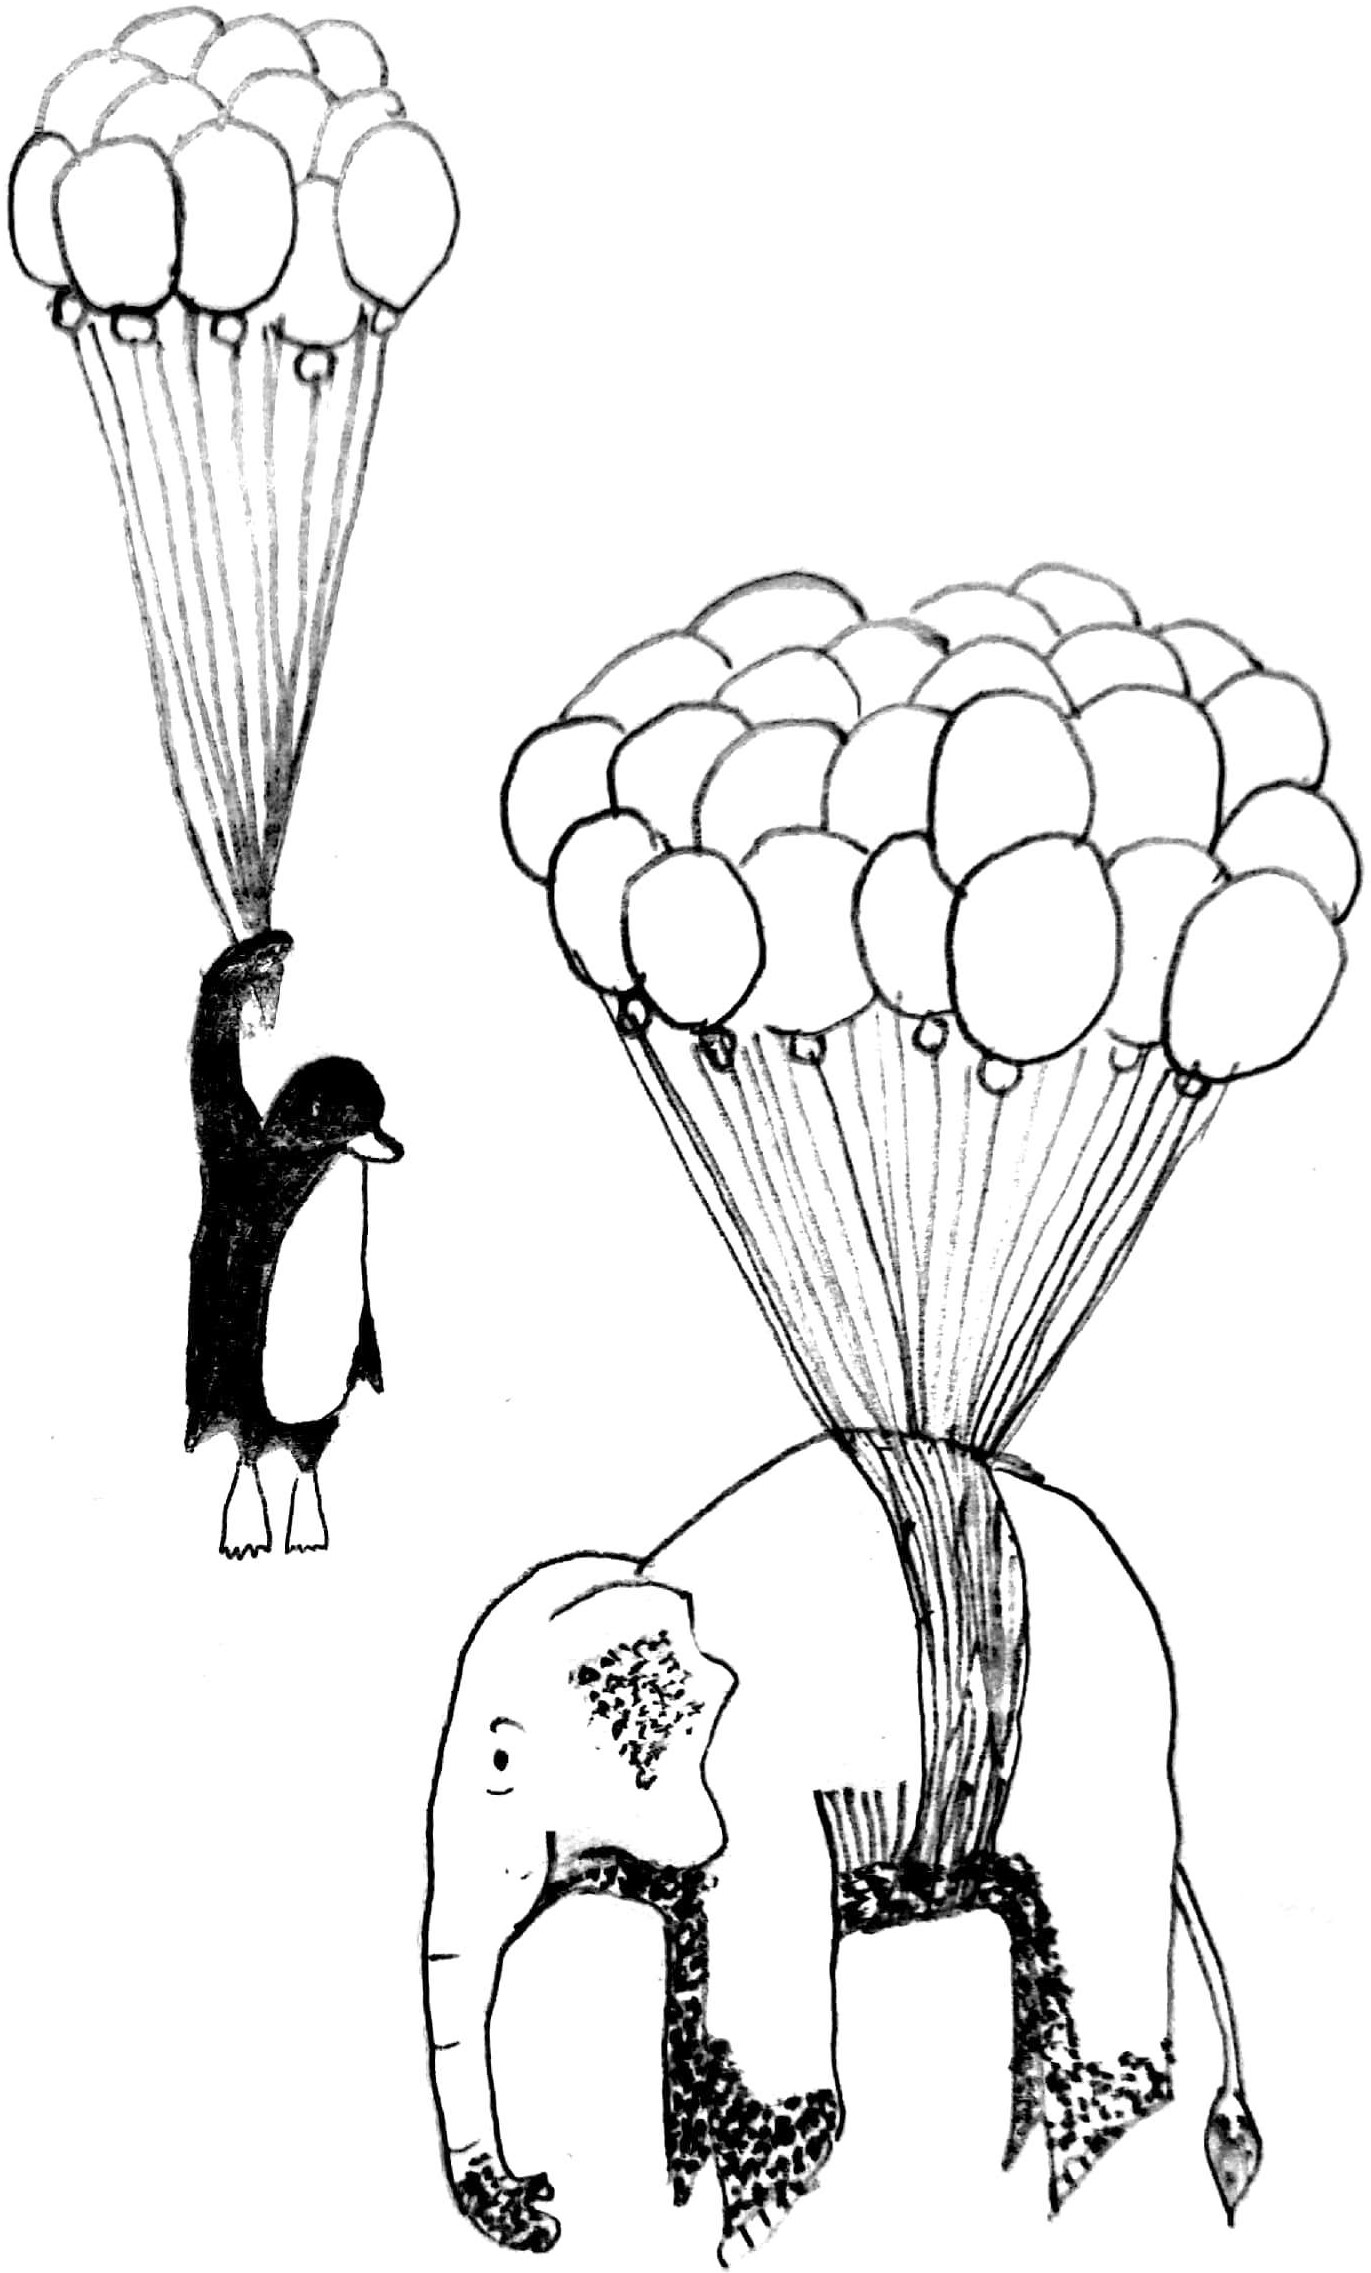
\includegraphics[width=45mm]{figures/bison/penguinelephant.jpg}\\\footnotesize\hphantom{.}\hfill---Sneha Khandelwal}

%     Mapping Neurons to Hardware
%       Sparsity
%           Expander, Iterative, Momentum
%       Quantize
%           Activation brevitas
%           Non Linear
Prototyping a neural network on a target hardware has a recurring cost, as often an engineer has no true estimate of the resources that will be required. This problem is further aggravated by the complex interaction of a topology and the underlying hardware, a compiler which translates the neural network to the target hardware typically yields inefficient deployment strategies.

In this thesis, we present a novel method of mapping neurons to hardware. This is done without the need for a custom accelerator architecture or a scheduler. If we turn back to our initial representation of a neuron as a boolean function $f: B^{ip} \rightarrow B^{op}$ where $B = \{0, 1\}$, we can hope to represent such a neuron with a look up table which requires $2^{ip} \times (op + ip)$ bits. Here, it becomes evident that in topology design, our most crucial design consideration should be to minimize $ip$, which is the number of input bits a neuron takes. However, as a neural network is essentially several layers of neurons placed sequentially, an implicit bound is also imposed upon $op$. While this may sound discouraging, a neural network is often heavily over-parametrized. The paper Deep Compression~\cite{han2015deep} used pruning, trained quantization and huffman coding to reduce the storage requirements of their neural networks by about $40\times$ without affecting their performance. 
\newthoughtpar{Prior works in accelerating neural networks}
There have been aggressive efforts in quantizing neural networks. Ever since Binary Neural Networks~\cite{courbariaux2016binarized} delivered respectable performance, FPGA implementations of quantized neural networks have been booming as well. \cite{umuroglu+:FPGA2017finn} proposed BNN accelerators with dataflow-style architectures (processing enginers instantiated at every layer). \cite{umuroglu+:FPGA2017finn} also implemented a folding scheme for larger neural networks so that they can be mapped to smaller devices. LUTs are heavily utilized in this implementation. \cite{wang2019lutnet} introduced LUTNet, which is a LUT optimized compression scheme which achieves very high LUT density. \cite{abdelsalam2018polybinn} introduced POLYBiNN, which utilized 110k 6-input LUTs to achieve an accuracy of $97.18\%$ on MNIST. POLYBiNN achieved 100M FPS on MNIST.
\section{Sparsity and Quantization}
\subsection{Sparsity}
In sparse neural networks, each neuron receives inputs from only a few connections of the previous layer. Often, it is beneficial to have regular sparsity, where pruning is done in a manner where neurons without value are pruned completely. This is not true for an LogicNet. We need to sparsify a network in a manner that every neuron maintains a small number of connections. This requirement has been demonstrated in \cref{fig:sparsify}. We identify three methods of Neural Network pruning: \textit{A-Priori Fixed Sparsity, Iterative Pruning and Learned Sparsity}. 
\marginpar{\centering
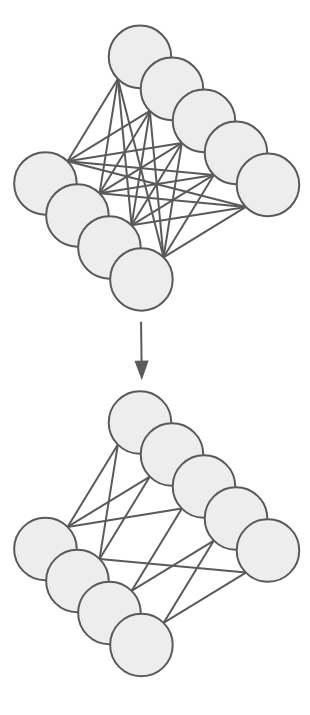
\includegraphics[width=120pt]{figures/bison/sparsify.png}
\captionof{figure}{Sparsification per neuron.}
\label{fig:sparsify}
% \endgroup
}
\newthoughtpar{A-Priori Fixed Sparsity}
We adapt concepts developed in Deep Expander Graphs~\cite{prabhu2018deep}. We use the concept of Random Expanders to explain our sparsity requirements. \\
\textbf{Random Expanders:} A random bipartite expander of degree $D$ on two Vertex Sets $U, V$ is a graph in which for every vertex $v \in V$, the $D$ neighbours are chosen independently and randomly from $U$.\\
We want to construct a neural network which corresponds to a sparse graph, where each vertex has $D$ neighbours. To extend this concept to convolutions, we need to view each set of convolutional kernels as one neuron, or as a vertex. This implies that for a convolutional filter set $(1, C, H, W)$, we can only have $D$ non-zero weights. 

\marginpar{\centering
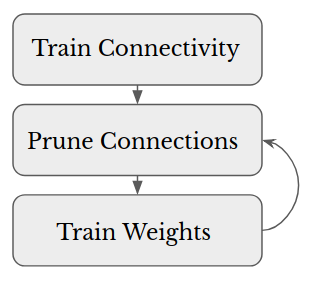
\includegraphics[width=120pt]{figures/bison/iterativepruning.png}
\captionof{figure}{Training Pipeline.}
\label{fig:iterativepruning}
% \endgroup
}
\newthoughtpar{Iterative Pruning}
Learning the right connections is an iterative process, the pruning is done by zero-ing the weights with the smallest magnitude. Pruning followed by retraining is one iteration, and per neuron pruning decay rates are calculated such that the number of weights zeroed out by the end of training gives rise to a fixed sparsity, where every neuron has $D$ neighbours. The training pipeline is presented in \cref{fig:iterativepruning}. Each iteration is greedy, and unlike the original implementation, we focus on pruning weights inside each neuron. This gives us a strict control over the connectivity of each neuron, consequently helping us in controlling the size of the truth table of the equivalent boolean function of the neuron. 

\newthoughtpar{Sparse Learning}
In the paper \textit{Sparse Networks from Scratch: Faster Training without Losing Performance}~\cite{dettmers2019sparse}, there are three steps; (a) Re-distribution of weights, (b) Pruning of weights, (c) Re-growing weights. To explain further, we take a simple $MLP$ model and index the layers as $l$, neurons as $n$ and synapses as $s$. The authors maintain an 'exponentially smoothed gradient' for every weight in the MLP. This can be described by the equation below.
$$
M_{l, n, s}^{t+1} = \alpha M_{l, n, s}^{t} + (1 - \alpha) \frac{\partial E}{\partial W_{l, n, s}}
$$
\newthoughtpar{Re-distribution of weights}
The normalized mean of the element-wise momentum for all non-zero weights in each layer is taken, as described below.
$$
M^{mean}_{l} = \frac{\sum_{n}\sum_{s} M_{l, n, s}}{\sum_{l}\sum_{n}\sum_{s} M_{l, n, s}}
$$
The resulting proportions are the momentum magnitude contributions for each layer. This is then used to calculate the number of weights to be regrown. For a network with sparsity $r$, the Regrowth for each layer is calculated below.
$$
Regrowth_{l} = n(Params)\times(1-r)\times M^{mean}_{l}
$$
\textbf{Pruning}\\
The authors prune a proportion $p$ (prune rate) of the weights with the lowest magnitude in each layer.\\
\textbf{Regrowth}\\
Weights are re-grown by enabling gradient flow of zero-valued weights which have the largest momentum magnitude.
\begin{figure}
    \centering
    \includegraphics[width=450pt]{figures/bison/neuronsparsity.png}
    \caption{This figure demonstrates the per neuron connectivity for a 3-Layer Neural Network.}
    \label{neuronsparsity}
\end{figure}
\newthoughtpar{Modifying Sparse Momentum Pruning}
As detailed in the \cref{algorithm1}, we had to make some notable changes to the Sparse Learning Algorithm. \cref{neuronsparsity} Attempts to measure the per-neuron fan-in for each neuron. Each divison in the X-Axis represents a Neuron, and each divison in the Y-Axis represents an incoming activation pixel. The dots represent which activation pixels each neuron is connected to. In the default sparse learning algorithm shown in \cref{neuronsparsity}, we can see that a few neurons have very high fan-in, while the others are pruned away. We desire a low, uniform per neuron fan in, which is achieved in the Modified Per Neuron Sparse Learning algorithm. 

% \includegraphics[width=450pt]{figures/bison/neuronsparsity.png}
% \begin{center}
% \captionof{figure}{This figure demonstrates the per neuron connectivity for a 3-Layer Neural Network. In the default sparse learning algorithm, we can see that a few neurons have very high fan-in, while the others are pruned away. We desire a low, uniform per neuron fan in, which is achieved in the Modifier Per Neuron Sparse Learning algorithm.}
% \end{center}
% \label{fig:neuronsparsity}



\begin{algorithm}
\caption{A Pruning Step for a L-Layer MLP}
 \hspace*{\algorithmicindent} \textbf{Input:} Layer $i$ to $l$ with: Momentum $M_{i}$; Weight $W_{i}$; binary $Mask_{i}$; prune rate $p$; Neuron Fan-in $F$; Neuron Prune $P1$; Neuron ReGrowth $R1$;\\
%  \hspace*{\algorithmicindent} \hspace{28pt} TotalMomentum $\leftarrow 0$; TotalNonzero $\leftarrow 0$;
 \hspace*{\algorithmicindent} \textbf{Output:} Updated weight $W^{t+1}$; TotalMomentum; TotalNonZero;
\begin{algorithmic}[1]
% \State Binarization of weights
\For{$i$ = 1 to $l$}
    \State MeanMomentum$_{i}$ $\leftarrow$ MeanMomentum$_{i}$ + $mean(abs(M_{i}[W_{i}\neq0]))$
    \State TotalMomentum $\leftarrow$ TotalMomentum + MeanMomentum$_{i}$
    \State NonZero$_{i}$ = $\sum(W_{i}\neq0)$
    \State TotalNonZero $\leftarrow$ TotalNonZero + NonZero$_{i}$
\EndFor
% \For{$i$ = 1 to $l$}
%     \State LayerContribution$_{i} \leftarrow$ MeanMomentum$_{i}$/TotalMomentum
%     \State $p_{i} \leftarrow$ getPruneRate($W_{i}, p$) 
% \EndFor
\For{$i$ = 1 to $l$}
    \For{Neuron in Layer $i$}
        \State Prune($P1$, Neuron)
        \State ReGrow($R1$, Neuron)
\EndFor
\EndFor
\end{algorithmic}
\label{algorithm1}
\end{algorithm}


\newthoughtpar{Discussion}
Our modification of the Sparse Learning Algorithm has some shortcomings. Due to the strict requirement of a fixed per-neuron Fan-in, the $MeanMomentum_{i}$ has no redistribution utility in our implementation. This implementation simply prunes weights per neuron by magnitude, and re-grows weights per neuron by their momentum. It is important to note that, in the future it may be a worthwhile endeavor to create a better re-distribution strategy which allows for variable fan-in per neuron based on the MeanMomentum per neuron. In our testing, such a re-distribution strategy had adverse effect on hardware cost, with very little to no gain in accuracy. We leave these loose ends as part of the algorithm so that the reader is aware of all the variables that are still being tracked in our implementation. 

    
\subsection{Quantization}
To support quantization, we utilize the Machine Learning PyTorch Library Brevitas~\cite{alessandro_pappalardo_2019_3525102}. Brevitas implements a set of building blocks to model a reduced precision hardware data-path at train time. Our methodology of design places no constraint on the weight data-type. We however, do have a constraint on the activation bit-width. We thus utilize the \textit{QuantReLU} and \textit{QuantHardTanh} layers to support Binary and uniform integer quantization of activations.
In a quantization flow with integer uniform quantization for activations, the bit-width together with the sign determines the min and max integer values used for scaling and clamping. Since the range of QuantReLU output is $QuantReLU(input) \in \mathbb{R}^{+}$, we do not have to worry about the sign bit for scaling. The \textit{QuantReLU} and \textit{QuantHardTanh} return a QuantTensor (NamedTuple), which propagate the following information:
\begin{itemize}
    \item quant\_tensor: The quantized tensor in dequantized representation (floating-point order of magnitude)
    \item scale\_factor: The scale factor of quant\_tensor
    \item bit\_width: The precision of quant\_tensor in bits.
\end{itemize}

\section{Quantifying Hardware Costs}
Now that we have discussed the ways we have tried to enforce sparsity and the quantization scheme being used, it is important to understand how sparsity and quantization work together to reduce the hardware cost for a neuron. We will deal with the implications of different sparsification and quantization methods on accuracy when we discuss the data-sets LogicNet was tested on.

\section{Research Recess  I -- Sparsity}

In the previous sections, we focused on methods to port neural networks of sizeable dimensions to the LogicNet topology. In spirit of research, a discourse on why some methods work, some don't could be of great value. 

\subsection{What are some methods to distribute non-zero weights?}
At first, this question may seem to have been answered already. While that is true to some extent, it is worth formalizing. The utility of exploring re-distribution methods is to find natural ways to make neurons adhere to specific fan-in constraints. In our A-Priori Fixed Sparsity methods, we have no focus on neuron importance. Our modified implementation of Sparse Learning algorithm simply clips off the same proportion of weights from each neuron. This may be very unnatural. We refer to the work by \cite{evci2019rigging} and consider two weight distribution strategies. The original work also considers an {Erd\H{o}s-R\'{e}nyi-Kernel} method, which is an extension of {Erd\H{o}s-R\'{e}nyi} method which takes the kernel size into consideration. 
\begin{itemize}
    \item \textit{Uniform:} The Sparsity of each layer is the same as the Total Sparsity.
    \item \textit{Erd\H{o}s-R\'{e}nyi:} The sparsity of each layer scales with 1 - $\frac{n^{l-1} + n{l}}{n^{l-1}\times n^{l}}$ where $n^{l}$ denotes the number of neurons at layer l. This method gives higher sparsity to layers with more parameters and lower sparsities to smaller ones.
\end{itemize}

\subsection{Ensembling and the {Erd\H{o}s-R\'{e}nyi} Method}
Ensembling has shown great benefits in our experiments, thus a way to take sparsity distribution in account and adjusting our model layer costs accordingly is an interesting exercise. 
We can benefit from the {Erd\H{o}s-R\'{e}nyi} method of weight redistribution, as it naturally aligns with our view of neural networks and allows them to scale a bit better. As the complexity of the LUT cost of a layer is$O(2^{B})$ (B is the fan-in in bits), if a layer with $N1$ neurons is made more sparse than a layer with $N2$ neurons where $N1>N2$. The LUT cost of the neurons become proportional to $2^{B1}{N1}$ and $2^{B2}{N2}$, note that as the sparsity of the larger layer is greater $\mathbb{E}(B2)>\mathbb{E}(B1)$. We thus allow ourselves to ensemble many of those smaller layers or the larger layers and balance the cost. The expression for the number of such smaller layers can be 'ensembled' can be provided by simply dividing the two LUT costs as to obtain $N2\frac{2^{B2-B1}}{N1}$. The inverse is true if the larger layer requires lesser LUTs. \\
We can also try adjusting the {Erd\H{o}s-R\'{e}nyi} method to take the exponential nature of the cost of a layer into account. To take this idea further, we do not need to proportionally ensemble intermediate layers, rather we can ensemble intermediate layers of arbitrary sizes as long as it respects the above proportionality in cost. Which in itself is only in place to have balanced sparsity between layers. What utility redistributing weights to balance sparsity across layers provides is an interesting research question.\\

\subsection{Is Sparsification Neural Architecture Search?}
If we think more closely about what we are doing, it becomes evident that for all our models, the maximum size of sparse models is bounded by the largest dense model we start with. This was pointed out by~\cite{evci2019rigging} and while it may seem trivial, it implies this statement not only from a parameter masking perspective but more interestingly, from a topological perspective. Some methods of Sparsification can be 'tagged' as Neural Architecture Search. It may make sense to look more closely at more 'esoteric' methodologies of discovering topologies which are sparse. We may tailor topologies ourselves, as we attempted in the previous subsction on \textit{Ensembling and the {Erd\H{o}s-R\'{e}nyi} Method}, or we can look at recent research in the field of discovering neural connections. Some of which are ~\cite{Wortsman2019DiscoveringNW} ~\cite{Mocanu_2018} ~\cite{liu2019sparse} ~\cite{bellec2017deep}. \\

The Sparse Evolutionary Training algorithm essentially replaces fully connected layers with Sparse Connected layers having the {Erd\H{o}s-R\'{e}nyi} topology. For each training epoch, they take each bipartite Sparse Connected layer, removing a fraction of the smallest positive and largest negative weights. They also randomly add new connections in the same amount as previously removed. \\
We need an algorithm that not only converts a fully connected layer to a Sparse Bipartite Graph, but treats each neuron with certain fan-in as nodes in a graph with arbitrary connectivity (without hierarchy). Ideally, we would like to implement a neural architecture search which does not pay heed to the hierarchial structure of DNNs. The search space for such a task is too huge. Sparsification of each neuron leads to a significantly smaller search space, but the order of complexity remains the same. \\
One of the most interesting papers which support such an idea is by \cite{Wortsman2019DiscoveringNW}. In this paper, a set of real edges $\eta$ is considered, with a set of \textit{hallucinated} edges $\xi_{hal} = V\times V \textbackslash \xi$. The magnitude of a weight is strengthened if the gradient pushes the activation in alignment with a certain edge. Over iterations, if it is strengthened enough it can join the set of real edges from the hallucinated edges. \\
It is extremely important to conduct this 'neural architecture search' in a manner such that the search space is navigated effectively. If the neural network has no 'hierarchy', it becomes a much harder task. Trying to discover sparse topologies which are not hierarchical in nature is one of the most exciting future areas of work for this thesis. 

% \begin{algorithm}
% \caption{A Pruning Step for a L-Layer MLP}\label{sparsemomentum}
%  \hspace*{\algorithmicindent} \textbf{Input:} Layer $i$ to $l$ with: Momentum $M_{i}$; Weight $W_{i}$; binary $Mask_{i}$; prune rate $p$; Neuron Fan-in $F$; Neuron Prune $P1$; Neuron ReGrowth $R1$;\\
% %  \hspace*{\algorithmicindent} \hspace{28pt} TotalMomentum $\leftarrow 0$; TotalNonzero $\leftarrow 0$;
%  \hspace*{\algorithmicindent} \textbf{Output:} Updated weight $W^{t+1}$; TotalMomentum; TotalNonZero;
% \begin{algorithmic}[1]
% % \State Binarization of weights
% \For{$i$ = 1 to $l$}
%     \State MeanMomentum$_{i}$ $\leftarrow$ MeanMomentum$_{i}$ + $mean(abs(M_{i}[W_{i}\neq0]))$
%     \State TotalMomentum $\leftarrow$ TotalMomentum + MeanMomentum$_{i}$
%     \State NonZero$_{i}$ = $\sum(W_{i}\neq0)$
%     \State TotalNonZero $\leftarrow$ TotalNonZero + NonZero$_{i}$
% \EndFor
% % \For{$i$ = 1 to $l$}
% %     \State LayerContribution$_{i} \leftarrow$ MeanMomentum$_{i}$/TotalMomentum
% %     \State $p_{i} \leftarrow$ getPruneRate($W_{i}, p$) 
% % \EndFor
% \For{$i$ = 1 to $l$}
%     \For{Neuron in Layer $i$}
%         \State Prune($P1$, Neuron)
%         \State ReGrow($R1$, Neuron)
% \EndFor
% \EndFor
% \end{algorithmic}
% \label{algorithm1}
% \end{algorithm}


% \begin{algorithm}
%  \For{$i$ in $[1,N_{iterations}]$}{
%   \For{all active connections $k$ $(\theta_k \geq 0)$}
%   {$\theta_k \leftarrow \theta_k - \eta \frac{\partial}{\partial \theta_k} \Eb - \eta \alpha + \sqrt{2 \eta T} \ \nu_{k}$\;
%   \textbf{if} $\theta_k < 0$ \textbf{then} set connection $k$ dormant \;
%   }
%   \For{all dormant connections $k$ $(\theta_k < 0)$}
%   {$\theta_k \leftarrow \theta_k + \sqrt{2 \eta T} \ \nu_{k}$\;
%   $\theta_k \leftarrow \max\{\theta_k, \theta_\text{min}\}$\;
%   \textbf{if} $\theta_k \ge 0$ \textbf{then} set connection $k$ active \;
%   }
%  }
%  \caption{Pseudo code of the soft-DEEP R algorithm. $\theta_\text{min}<0$ is a constant that defines a lower boundary for negative $\theta_k$s.}
%  \label{alg:sdeepr}
% \end{algorithm}




% /*
% Introduction
% The need for accelerators
%     CPUs, GPUs, ASICs, FPGAs.
% Background
%     FPGA and HW/SW Co-Design
%     Mapping Neurons to Hardware
%       Sparsity
%           Expander, Iterative, Momentum
%       Quantize
%           Activation brevitas
%           Non Linear
% LogicNet: A Library for Mapping HBBs to NEQs
%     Introduction
%     Components
%       Linear
%       Convolutions
%     Design Automation
%       TruthTableGen
%       VerilogGen
%       Synthesis
% Testing LogicNet
%     LogicNet4HEP
%       Introduction
%       Models
%     MNIST 
%       Models
% Concluding Remarks
%     Research Questions
%     Conclusion
% */